\begin{figure}[tbp]
\begin{center}
\includegraphics[width=0.48\textwidth]{figure/sn_z1_z2.eps}
\end{center}
\vspace{-0.7cm}
\caption{Cumulative S/N, assuming Planck noise at 217 GHz, $f_{sky}=0.8$. 
}
\label{fig:sn}
\end{figure}
%In real surveys, when we calculate the cross angular power spectrum $C_\ell$ between reconstructed kSZ signals and CMB measurements, we will have to face statistical errors. 
%They can be approximated as:
In this Section, we consider our ability to distinguish the kSZ effect from the primary CMB and instrumental noise. We estimate the signal-to-noise for the kSZ effect as:
%\begin{eqnarray}
 %   \frac{\Delta C_\ell}{C_\ell}\simeq \frac{1}{r\sqrt{(2l+1)\Delta l f_{sky}}}\sqrt{\frac{C_\ell^{\mr{CMB}}+C_\ell^{kSZ}+C_\ell^{\mr{CMB},N}}{C_\ell^{kSZ,\Delta z}}(1+\frac{C^N_{\hat \Theta}}{C_{\hat \Theta}})}\,
%\end{eqnarray}
\begin{eqnarray} 
\label{eq:sn}
    \frac{S}{N}&=&\frac{C_\ell}{\Delta C_\ell}\\\nonumber
               &\simeq&
    r\sqrt{(2\ell+1)\Delta l f_\mathrm{sky}}\sqrt{\frac{C_\ell^{\mathrm{kSZ},\Delta z}}{C_\ell^{\mr{CMB}}+C_\ell^\mathrm{kSZ}+C_\ell^{\mr{CMB},N}}},
\end{eqnarray}
where $C_\ell^\mathrm{CMB}$ is the angular power spectrum of primary CMB, $C_\ell^\mathrm{CMB,N}$ is the contribution to the covariance from instrumental noise, $C_\ell^{\mathrm{kSZ},\Delta z}$ is the kSZ signal from within a certain redshift bin,  
$r$ is the correlation coefficient defined in Eq.(\ref{eq:r}), and $f_\mathrm{sky}$ is the percent of sky area covered by both the CMB and 21 cm IM surveys.

Notice that the S/N is related to the cross correlation coefficient we could obtain from 21cm IM and the 
relative strength of kSZ signals as opposed to primary CMB and facility noise.

In this paper, $C_\ell^\mr{CMB}$ is calculated using CAMB \cite{CAMB}. $C_\ell^\mr{CMB,N}$ is estimated with Planck data \cite{Planck2015} at 217GHz, with sensitivity per beam solid angle given by $\sigma_{p,T}=8.7\mu K_\mathrm{CMB}$ and an effective beam full-width-half-maximum of $\theta_\mathrm{FWHM}\sim 5'$. 
We assume sky coverage $f_\mathrm{sky}=0.8$. $C_\ell^{\mathrm{kSZ},\Delta z}$ is calculated within two bins of size 1200 Mpc/h, centered at redshift 1 $\&$ 2, respectively. 
The cumulative S/N calculated using Eq. \eqref{eq:sn} is shown in Fig.\ref{fig:sn}. The S/N at $z=2$ is higher than $z=1$ due to the high electron density, and the overall S/N should well reach 50 with HIRAX. With Planck noise levels, the resolution of HIRAX already covers the most important $\ell$. 
%It goes into larger scale of baryon distribution than 
%other tracers proposed. 
